%!TEX program = lualatex
\documentclass[masterarbeit,grey, english]{mas-thesis-sections}	% Available options:
															% masterarbeit, bachelorarbeit, dissertation,
															% masterprojekt, bachelorprojekt, seminararbeit,
															% fallstudie, grey (für Graustufen), english

\author{Max~Mustermann}						% ~ for nicer spaces
\authoraddress{Musterstr.~90\\12345 Essen}
\matrikelnumber{2251234}
\title{Titel~der~Arbeit}
\supervisor{Univ.-Prof.~Dipl.-Ing.~Dr.~Betreuer~Name}
\reviewerA{Univ.-Prof.~Dr.~Tobias~Hoßfeld}
\reviewerB{Gutachter~B}
\degreecourse{Angewandte Informatik~-~Network Engineering}
\location{Essen}
\handoverdate{23.10.2016}
\semester{Wintersemester~2016/2017}


%% load bibs
\addbibresource{bibliography/bibliography.bib}
%\addbibresource{bibliography/more-bibliography.bib}

%\DeclareBibliographyCategory{ownpub}

%%%%%%%%%%%%%%%%%%%%%%%%%%%%%%%%%%%%%%%%%%%%%%%%%%%%%%%%%%%%%%%%%%%%%%%%%%%%%%%%
\begin{document}

\maketitle				% Title Page

%
% An optional license. You can change the CC license in the mas-thesis-common.cls
% or remove this entirely.
%
\makelicensepageCCBYSA

\cleardoublepage


% Only necessary for dissertation, masterarbeit and bachelorarbeit
\eidesstattlicheErklaerung

\pagenumbering{Roman}
\phantomsection
% Set to either section or chapter depending on chosen template
\addcontentsline{toc}{section}{Contents}%
\tableofcontents		% Table of Contents

\cleardoublepage

\listofillustrations	% List of Figures and List of Tables


\cleardoublepage

\newpage
\begingroup % printglossar{y,ies} forces a cleardoublepage between glossaries and after it, we supress this here
	\let\clearpage\relax
	\printglossaries
\endgroup

\pagenumbering{arabic}
\setcounter{page}{1}

% Optional input if the thesis should be split into different files

% \input{components/license.tex}
% \input{components/toc.tex}
% \input{components/indices.tex}
% \input{components/quote.tex}
% \input{components/abstract.tex}
% \input{components/acknowledgments.tex}

%\chapter{Introduction}	% Remove if not dissertation or masterarbeit

\section{Abstract}

This document is a short example of how to use this template to write your own thesis. It gives a brief summary of the most important aspects and options that define this template.

\newpage


\section{General}

There are 2 differnt class files available: mas-thesis-sections and mas-thesis-chapters. Use the first if you plan to write a short thesis like a Bachelor Project or a Case Study and ignores chapters for the most past. The latter is better suited for a Master Thesis or Dissertation because it allows you to divide your thesis better. But nothing stops you to devide your Bachelor Thesis in chapters if you think that it will fit.

\newpage


\section{Sections}

This is an example of a numbered section. The section number increases automatically and does not need to be stated. To use a unnumbered section, just use \texttt{\textbackslash section* \{Name of unnumbered section\}}. A section can be divided by multiple subsections.

\subsection{Subsections}

This is a numerated \texttt{\textbackslash subsection}. There is also a \texttt{\textbackslash subsubsection} command. To create an unnumbered subsection, just add * like needed for sections.

\subsubsection{Subsubsection}

And while we're at it, here's a sub-sub-section for you!

\paragraph{A paragraph} is you! But there are no dragons, sorry about that.

\newpage

\section{Imports}

Large thesis like master thesis and dissertations often get very confusing when written in single document. You can import other .tex files with the\\\texttt{\textbackslash include\{other-latex-file.tex\}} command. The formatting will be taken from the master file and the sections, figures, tables, footnotes, citations, etc. are integrated in the context of the master file.

\newpage


\section{Tables and Figures}

In \LaTeX\ you can use tables and figures which will be automatically added to the List of Tables and List of Figures after the Table of Contents.

\subsection{Tables}

\begin{table}[ht]
\begin{center}
	\begin{tabular}{ l | c | r }
		1 & 2 & 3 \\
		\hline
		4 & 5 & 6 \\
		7 & 8 & 9 \\
	\end{tabular}
	\caption{Example of a table}
	\label{table:1}
\end{center}
\end{table}

\subsection{Figures}

Figures should be vector graphics where possible. \LaTeX can parse PDF and EPS out of the box but SVG can also be used with the svg package. If no vector graphics are available and you need to include raster graphics like JPEG, PNG, or BMP, make sure you have a high resolution and high DPI image. Note that the resulting PDF file can be very large when using a lot of raster graphics.

\begin{figure}[ht]
	\centering
	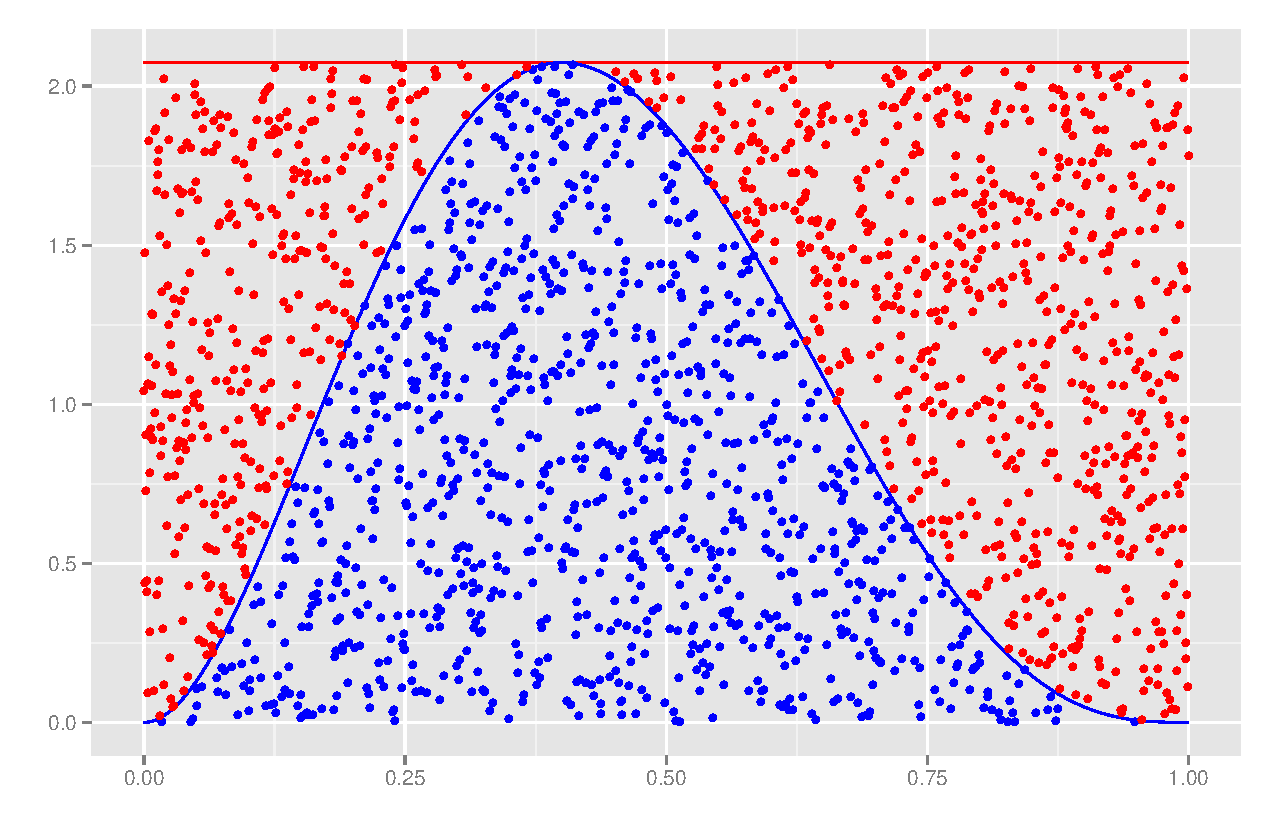
\includegraphics[height=5.1cm]{graphics/demo-graphic.pdf}
	\caption{Example of an imported PDF graphic}
	\label{figure:1}
\end{figure}

\newpage

\section{Bib\TeX\ and Footnotes}

Every thesis contains references. With Bib\TeX\footnote{\url{http://www.bibtex.org}} you can easily define them in one or more files and load them with \LaTeX\ and cite them at any time.\cite{exampleBook}
\cleardoublepage

\printbibliography[heading=bibintoc]



\end{document}
